\chapter{Architetture Parallele}

Per aumentare ancora di più le prestazioni, se è già stato applicato tutto ciò descritto in precedenza, si deve ricorrere a un'architettura dotata di più unità computazionali in modo da avere un \fancyglitter{parallelismo esplicito}. 

\nt{Preso in considerazione il fatto che i programmi debbano andare riscritti per girare su più core.}

\section{I Problemi del Parallelismo Esplicito}

Tuttavia, (eccetto che in casi molto molto particolari) l’incremento di
prestazioni (il cosiddetto \fancyglitter{speed-up}) che si può ottenere usando più
CPU su cui far girare in parallelo i vari programmi è meno che
lineare rispetto al numero di CPU disponibili. Principalmente perché i programmi che girano in parallelo dovranno sincronizzarsi tra loro. Consideriamo il comando "gcc main.c function1.c function2.c -o output". Supponiamo che, lanciando il programma su una macchina monoprocessore ci vogliano 7 secondi: 

\begin{itemize}
  \item 3 secondi per compilare main.c 
  \item 2 secondi per compilare function1.c 
  \item 1 secondo per compilare function2.c 
  \item 1 secondo per linkare gli oggetti. 
\end{itemize}

\paragraph{}
Con 3 CPU a disposizione i tre sorgenti possono essere compilati in parallelo, ma l'operazione di linking può essere eseguita solo dopo che tutti e tre gli oggetti sono stati generati (quindi dopo 3 secondi). In questo modo il tempo si riduce da 7 a 4 secondi con uno speed-up di 1.75 pur avendo usato 3 processori.
\begin{figure}[h]
    \centering
    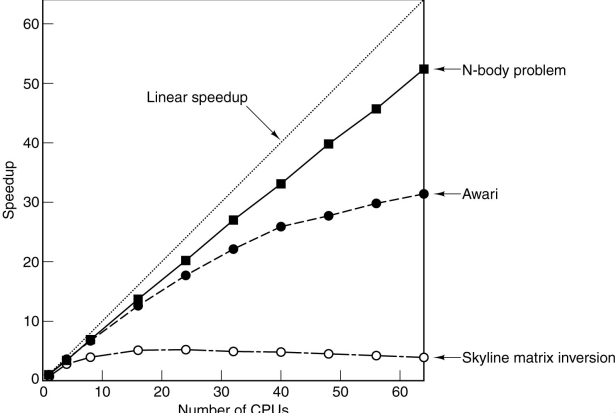
\includegraphics[width=0.3\textwidth]{04-ArchitettureParallele/speed-up.png}
    \caption{Speed-up di alcuni problemi computazionali.}
\end{figure}
\pagebreak
\begin{figure}[!h]
    \centering
    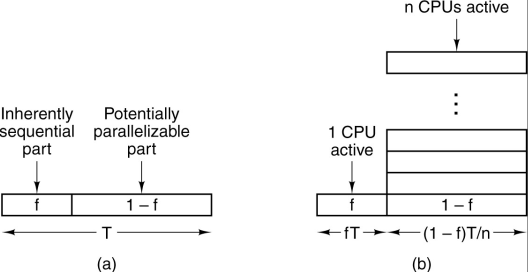
\includegraphics[scale=0.7]{04-ArchitettureParallele/Parallelizzazione limiti.png}
    \caption{Sia P un programma che gira in tempo T su una CPU, con f = la
frazione di T dovuta a codice sequenziale, e (1-f) la frazione di T
dovuta a codice parallelizzabile.}
\end{figure}

\nt{Il tempo di esecuzione dovuto alla parte parallelizzabile, passa
da (1-f)T a (1-f)T/n se sono disponibili n processori. Questa è nota come \fancyglitter{legge di Amdahl}}

\begin{figure}[h]
    \centering
    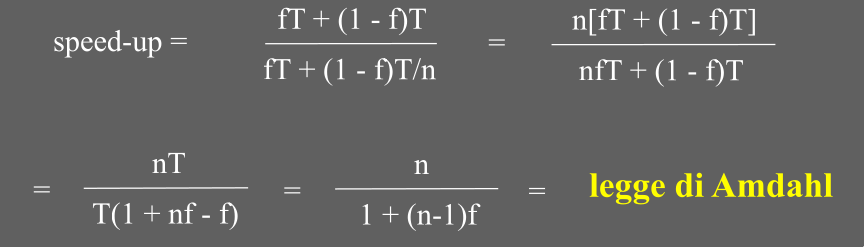
\includegraphics[scale=0.5]{04-ArchitettureParallele/Legge di Amdahl.png}
    \caption{La legge di Amdahl.}
\end{figure}

\begin{itemize}
  \item Se si vuole ottenere uno speed-up perfetto, pari al numero di CPU usate, f deve valere 0, ma ciò è impossibile. 
  \item Spesso il miglioramento è sub-lineare.
\end{itemize}

\paragraph{I problemi del parallismo esplicito sono generalmente due:}

\begin{enumerate}
  \item La quantità limitata di parallelismo nel codice dei programmi (problema software). 
  \item Gli elevati costi delle comunicazioni tra processori e memoria (problema hardware).
\end{enumerate}

\nt{Per molte applicazioni avere uno speed-up, seppur limitato, è comunque accettabile, perché: 
\begin{itemize}
  \item La presenza di più processori aumentà l'affidabilità del sistema. 
  \item Servizi che per loro natura sono forniti su ampia scala geografica,
devono essere implementati con una architettura distribuita. Se il
sistema fosse centralizzato in un unico nodo, l’accesso di tutte le
richieste a quest’unico nodo costituirebbe probabilmente un collo
di bottiglia in grado di rallentare enormemente il servizio fornito.
\end{itemize}
}

\paragraph{Ci sono tre tipi di architetture parallele esplicite:}

\begin{itemize}
  \item Multi-threading (a). 
  \item Sistemi a memoria condivisa (b, c). 
  \item Sistemi a memoria distribuita (d, e).
\end{itemize}

\begin{figure}[h]
    \centering
    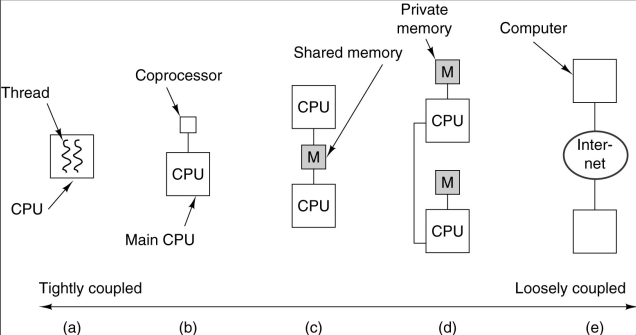
\includegraphics[scale=0.5]{04-ArchitettureParallele/PE.png}
    \caption{Vari tipi di architetture esplicitamente parallele.}
\end{figure}

\section{Multi-Threading}

\subsection{Introduzione}

\dfn{Architettura Multi-Threaded}{
  Una CPU multi-threaded è una architettura parallela un po’
particolare, in quanto il multi-threading è realizzato con un’unica
CPU (sempre single core), ma porta il programmatore
a concepire e sviluppare le sue applicazioni come formate da un
insieme di programmi che possono essere eseguiti in parallelo:
i thread.
}

\nt{Se questi programmi vengono fatti girare su una CPU che supporta il multi-threading ne sfrutteranno le caratteristiche architetturali.}

\paragraph{}

L’idea del multi-threading nasce dalla constatazione di un problema
di fondo presente in qualsiasi CPU pipelined: un cache miss
produce una “lunga” attesa necessaria per recuperare l’informazione
mancante in RAM. Se non c’è un’altra istruzione indipendente da poter eseguire,
o se non è implementato lo scheduling dinamico della pipeline,
la pipeline va in stall. Una soluzione per non sprecare inutilmente cicli di clock in attesa
del dato mancante è il multithreading: permettere alla CPU di
gestire più peer-thread allo stesso tempo: se un thread è bloccato
la CPU ha ancora la possibilità di eseguire istruzioni di un altro
thread, in modo da tenere le varie unità funzionali comunque
occupate.

\clm{}{}{
  \begin{itemize}
    \item Per implementare il multithreading, la CPU deve poter gestire lo
stato della computazione di ogni singolo thread. 
\item Ci deve essere un Program Counter (PC) e un set di registri separato per ciascun thread.  
\item Il thread switch deve essere più efficiente del process switch.
  \end{itemize}
}

\subsection{Tipi di Multi-Threading}

\paragraph{Esistono due tecniche di base per il multi-threading:}

\begin{itemize}
  \item \fancyglitter{Fine-grained multi-threading}. 
  \item \fancyglitter{Coarse-grained multi-threading}.
\end{itemize}

\dfn{Fine-grained Multi-Threading}{
  Lo switching tra i vari peer-thread
avviene ad ogni istruzione, indipendentemente dal fatto che
l’istruzione del thread in esecuzione abbia generato un cache miss.

Lo \newfancyglitter{scheduling} tra i vari peer-thread avviene secondo una politica round robin e la CPU deve essere in grado di effettuare lo switch praticamente senza overhead (che sarebbe inaccettabile).
}
\nt{Se vi è un numero sufficiente di peer-thread, è possibile che ve ne
sia sempre almeno uno non in stall, e la CPU può essere mantenuta
sempre attiva.}

\clm{}{}{
\begin{itemize}
  \item Lo stalling della CPU può anche essere dovuto a una dipendenza o a un branch, poiché l'ILP dinamico non può sempre evitarlo.
  \item Invece, con il Fine-grained multithreading, in un'architettura pipelined, se: 
    \begin{itemize}
      \item La pipeline ha $k$ stage. 
      \item Ci sono almeno $k$ peer-thread da eseguire. 
      \item La CPU esegue lo switch tra thread a ogni ciclo di clock.
    \end{itemize}
  \item Non ci può essere mai più di un'istruzione per thread nella pipeline in un dato istante, le dipendenze sui dati vengono risolte automaticamente e la pipeline non va mai in stall (se un cache miss può essere gestito in un numero di cicli di clock inferiore o uguale al numero di thread in esecuzione).
\end{itemize}
}

\begin{figure}[h]
    \centering
    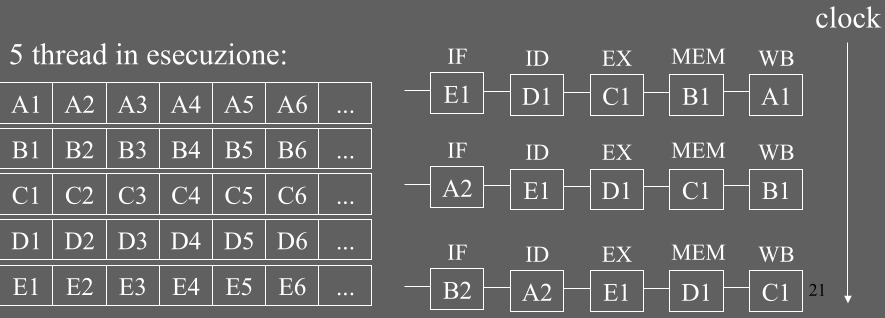
\includegraphics[scale=0.5]{04-ArchitettureParallele/fine.png}
    \caption{Fine-grained multithreading in una CPU con pipeline
     a 5 stadi.}
\end{figure}

\nt{Lo scheduling Fine-grained fa si che un thread venga rallentato anche quando potrebbe proseguire l'esecuzione perché non sta generando alcuno stall (per via del fatto che vada eseguito un context switch a ogni istruzione). Inoltre potrebbero esserci meno thread che stage della pipeline, per cui non è facile mantenere la CPU sempre occupata.}

\dfn{Coarse-grained Multi-Threading}{
Lo switch avviene solo quando il
thread in esecuzione genera uno stall, provocando così lo spreco di
un ciclo di clock.

Viene effettuato lo switch a un altro thread. Quando anche questo genererà uno stall verrà schedulato un terzo thread (o eventualmente si tornerà al primo) e così via. 
}

\nt{Questo approccio spreca potenzialmente più cicli di clock rispetto al Fine-grained, perché comunque lo switch avviene solo se si è verificato uno stall. Ma se ci sono pochi thread attivi questi possono essere sufficienti per tenere la CPU occupata.}

\paragraph{Fine-grained vs. Coarse-grained:}

\begin{itemize}
  \item Non è pensabile che lo switch tra thread possa avvenire senza perdite di tempo.
  \item Se le istruzioni dei vari thread non generano stall molto frequentemente uno scheduling Coarse-grained è più vantaggioso (perché il Fine-grained, ogni ciclo di clock, paga un overhead limitato, ma non nullo).
  \item Fine-grained $\rightarrow$ Sistema operativo time-sharing. 
  \item Coarse-grained $\rightarrow$ Sistema operativo multitasking.
\end{itemize}

\dfn{Medium-grained Multi-Threading}{
  Una via di mezzo tra il fine- e il
coarse- grained multithreading consiste nell’eseguire lo switch tra
thread solo quando quello in esecuzione sta per eseguire una
istruzione che potrebbe generare uno stall di lunga durata,
come ad esempio una load (che potrebbe richiedere un dato non
in cache), o un branch (perché anche l'istruzione nel caso il branch venisse preso potrebbe non trovarsi nelle cache L1, L2, L3).

L'istruzione viene avviata, ma il processore esegue in ogni caso lo switch a un altro thread.
}

\nt{In questo modo non si spreca neanche il ciclo di clock dovuto all'eventuale stall dell'istruzione eseguita (come accade nel Coarse-grained).}

\qs{}{Ma come si fa a sapere a quale thread appartiene una qualsiasi
istruzione nella pipeline?}

\begin{itemize}
  \item Nel caso del Fine-grained Multi-Threading l'unico modo è di attaccare un \fancyglitter{thread identifier} a ogni istruzione. Per esempio l'ID univoco associato a quel thread all'interno dell'insieme di peer-thread a cui appartiene. 
  \item Nel caso del Coarse-grained Multi-Threading si può adottare la stessa soluzione oppure si può anche svuotare la pipeline a ogni thread switch (in questo modo le istruzioni di un solo thread alla volta sono nella pipeline e quello sa sempre a quale thread appartengono). 
\end{itemize}

\nt{Ciò ha senso solo se lo switch avviene a intervalli molto maggiori del tempo necessario a svuotare la pipeline. Inoltre, le istruzioni dei vari thread, devono essere, per quanto possibile, tutte contemporaneamente nella cache delle istruzioni, altrimenti ogni context switch tra thread produce un cache miss e si perde qualsiasi vantaggio nell'utilizzare i thread.}

\subsection{Simultaneous Multi-Threading}

Le moderne \fancyglitter{architetture superscalari}, multiple issue e a scheduling dinamico della pipeline danno la possibilità di sfruttare contemporaneamente il parallismo insito nelle istruzioni di un programma (ILP) con il parallelismo insito in un insieme di peer-threads: il Thread Level Parallelism (TLP). 

\begin{center}
  \fancyglitter{ILP + TLP = SMT (Simultaneous Multi-Threading)}
\end{center}

\nt{Le ragioni per implementare SMT risiedono nell'osservazione che le moderne CPU multiple issue hanno più unità funzionali di quante siamo mediamente sfruttabili dal singolo thread in esecuzione. 

Sfruttando il register renaming e lo scheduling dinamico istruzioni appartenenti a thread diversi possono essere eseguite insieme.
}

\begin{figure}[h]
    \centering
    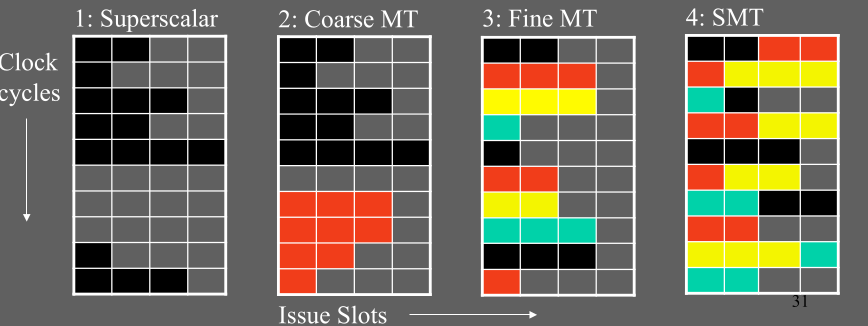
\includegraphics[scale=0.5]{04-ArchitettureParallele/SMT.png}
    \caption{Confronto tra processori.}
\end{figure}

\clm{}{}{
  \begin{itemize}
    \item Anche nel SMT non si riesce sempre ad avviare il massimo numero possibile di istruzioni per ciclo di clock a causa del numero limitato di unità funzionali e di stazioni di prenotazione disponibili, della capacità della cache di istruzioni di fornire le istruzioni dei vari thread e del numero di thread presenti. 
    \item SMT può essere adeguatamente supportato solo se sono disponibili registri rinominabili in abbondanza. 
    \item Nel caso di una CPU che supporti la ridenominazione sarà importante avere un ROB distinto per ogni thread in modo da gestire in maniera indipendente i commit.
  \end{itemize}
}

\subsubsection{Il Multi-Threading Intel}

\dfn{Hyperthreading}{
  Viene supportata l’esecuzione di due thread in modalità SMT.
}

\clm{}{}{
  \begin{itemize}
    \item Dal punto di vista del Sistema Operativo, una CPU multithreaded
è vista come due CPU che condividono cache e RAM: dunque due
applicazioni che condividono lo stesso spazio di indirizzamento,
possono essere eseguite in parallelo nei due thread. 
\item Siccome due thread possono usare contemporaneamente la CPU,
occorre adottare delle strategie per fare in modo che entrambi i
thread possano utilizzare le varie risorse della CPU.
  \end{itemize}
}

\paragraph{\fancyglitter{Ci sono 4 strategie ideate da Intel:}}

\begin{itemize}
  \item \fancyglitter{Risorse duplicate:} quelle necessarie a gestire l'esecuzione dei due thread (due program counter e due banchi di registri separati). 
  \item \fancyglitter{Risorse partizionate equamente tra i due thread:} la coda delle microistruzioni e il ROB. 
  \item \fancyglitter{Risorse condivise dinamicamente:} un thread può occupare quante linee di cache vuole, eventualmente rallentando l'altro thread. 
  \item \fancyglitter{Risorse condivise dinamicamente:} lo scheduler che invia le uops alle varie stazioni di prenotazione. 
\end{itemize}

\begin{figure}[h]
    \centering
    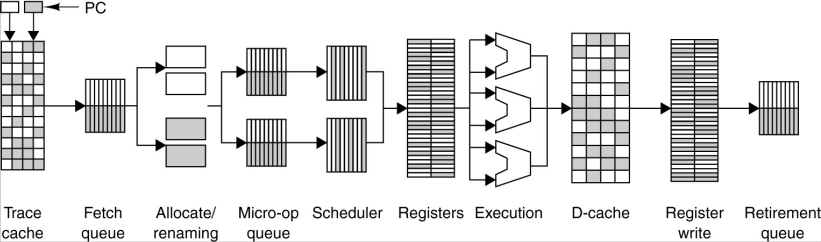
\includegraphics[scale=0.5]{04-ArchitettureParallele/Intel.png}
    \caption{Risorse in una CPU Intel.}
\end{figure}

\paragraph{Brevi note storiche:}

\begin{itemize}
  \item Intel abbandona la tecnologia Hyperthreading nel passaggio ai nuovi processori dual core (non supportavano il multithreading). 
  \item L'Hyperthreading è stato reintrodotto a partire dal 2008 con l'architettura Nehalem. 
  \item IBM Power 7 (2010) implementò SMT con 4 thread contemporaneamente attivi. 
  \item I processori UltraSPARK, da T2 in poi, supportano il Fine-grained multithreading con 8 thread per core. L'UltraSPARK T1 solo 4 thread per core.
\end{itemize}

\section{Multiprocessori a Memoria Condivisa}

\subsection{Introduzione}

\dfn{Multiprocessore}{
  Un \newfancyglitter{multiprocessore} è un'architettura con più CPU che condividono la stessa memoria primaria. 
 }
 \subsubsection{}
 In un sistema multiprocessore tutti i processi che girano sulle varie CPU condividono un unico spazio di indirizzamento logico, mappato su una memoria fisica che può però anche essere distribuita tra i vari banchi di memoria in modi diversi. Ogni processo può leggere e scrivere un dato in memoria specificando un indirizzo usato da LOAD e STORE, e la comunicazione tra processi avviene attraverso la memoria condivisa.


 \nt{È responsabilità dell’hardware del sistema fare in modo che tutte
le CPU possano vedere e usare la stessa memoria principale.}

\begin{figure}[h]
    \centering
    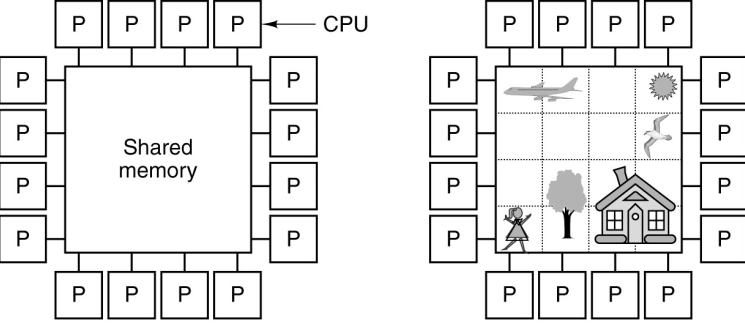
\includegraphics[scale=0.5]{04-ArchitettureParallele/Multi.png}
    \caption{Schema di base di un multiprocessore.}
\end{figure}

\clm{}{}{
  \begin{itemize}
    \item Siccome tutte le CPU vedono lo stesso spazio di indirizzamento,
è sufficiente una copia del sistema operativo. 
\item Quando un processo termina o va in wait per qualche ragione, il
S.O. può cercare nella coda di ready un altro processo a cui dare la
CPU idle. 
\item Al contrario, nei sistemi a memoria non condivisa, ogni CPU deve
far girare la propria copia del sistema operativo, e i processi
possono comunicare solo attraverso lo scambio di messaggi. 
\item Il problema di fondo dei sistemi multiprocessore a memoria
condivisa è la memoria stessa, che è difficile da far funzionare
in maniera efficiente quanto più è alto il numero dei processori
coinvolti.
  \end{itemize}
}

\qs{}{Come funzionano i sistemi multiprocessore?}

\begin{itemize}
  \item Tutti i moderni SO (Windows, Solaris, Linux, MacOS) prevedono in
particolare la cosiddetta multielaborazione simmetrica (symmetric
multiprocessing, SMP), in cui (tralsciando un po’ di cose) uno
scheduler gira su ciascun processore. 
\item I processi “ready to run” possono essere inseriti in un’unica coda,
vista da ciascun scheduler, oppure vi può essere una coda “ready to
run” separata per ciascun scheduler/processore. 
\item Quando lo scheduler di un processore si attiva, sceglie uno dei
processi “ready to run” e lo manda in esecuzione sul proprio
processore.
\item Un aspetto importante dei sistemi multiprocessore è il bilanciamento
del carico.
\item Non ha infatti senso avere un sistema con più CPU se poi i vari
processi da eseguire non sono distribuiti più o meno omogeneamente
tra i vari processori. 
\item Nel caso di un’unica coda ready to run, il bilanciamento del carico
è solitamente automatico: quando un processore è inattivo, il suo
scheduler prenderà un processo dalla coda comune e lo manderà in
esecuzione su quel processore.
\item I SO moderni predisposti per l’SMP usano però spesso una coda
separata per ciascun processore in modo da non doversi sincronizzare
per accedere all’unica coda di ready quando devono inserire o
prelevare un processo dalla coda. Esiste allora un esplicito meccanismo di bilanciamento del carico
che può prendere un processo in attesa sulla coda di un processore
sovraccarico e spostarlo nella coda di un processore scarico\footnote{Per esempio, in Linux SMP meccanismo di bilanciamento del carico
si attiva ogni 200 millisecondi, e ogni qualvolta si svuota la coda di
un processore.}.
\end{itemize}

\subsection{UMA}

Esistono sostanzialmente due classi di architetture multiprocessore: 

\begin{itemize}
  \item \fancyglitter{UMA}. 
  \item \fancyglitter{NUMA}.
\end{itemize}

\nt{Una terza classe, detta \fancyglitter{COMA} (Cache Only Memory Architecture), sebbene teoricamente promettente non è stata mai implementata in maniera soddisfacente.}

\dfn{UMA}{
  Uniform Memory Access (UMA) è un tipo di architettura in cui tutti i processori condividono un'unica memoria primaria centralizzata e quindi ogni CPU ha lo stesso tempo di accesso alla memoria. 
}

\nt{Questi sistemi vengono anche chiamati SMP (Symmetric Shared-Memory Multiprocessor)}

\begin{figure}[h]
    \centering
    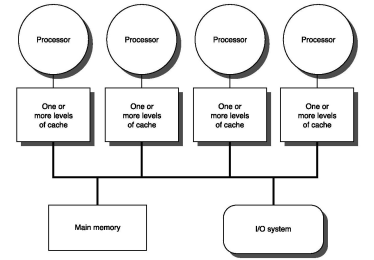
\includegraphics[scale=0.6]{04-ArchitettureParallele/UMA.png}
    \caption{Schema UMA.}
\end{figure}

\clm{}{}{
  \begin{itemize}
    \item I sistemi multiprocessore UMA costituiscono il primo tipo di
sistemi multiprocessore, e nella sua forma più semplice un sistema
UMA prevede un unico bus su cui si affacciano almeno due CPU e
una memoria (condivisa da tutti i processori). 
\item Quando una CPU vuole leggere una locazione di memoria verifica
prima che il bus sia libero, invia la richiesta al modulo di interfaccia
della memoria e attende sul bus che arrivi il valore richiesto. 
\item La memoria condivisa può però facilmente diventare un collo di
bottiglia per le prestazioni del sistema, visto che tutti i processori
devono sincronizzarsi sull’uso di un singolo bus e memoria. 
  \end{itemize}
}

\nt{I moderni processori multi-core sono semplici architetture UMA in cui la prima cache condivisa da tutti i core (solitamente L3) costituisce un canale di comunicazione più efficiente della RAM: se un core modifica un dato un altro core potra vedere la modifica in una linea di L3 anziché dover arrivare fino alla linea di RAM corrispondente.}

\begin{figure}[h]
    \centering
    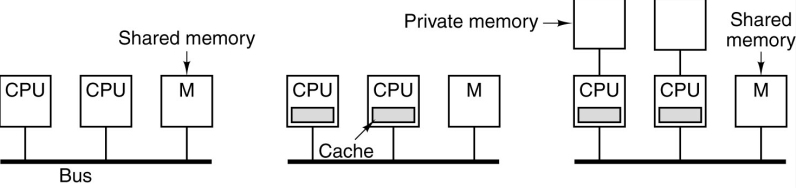
\includegraphics[scale=0.5]{04-ArchitettureParallele/memory.png}
    \caption{Ogni processore dispone di una sua memoria privata.}
\end{figure}

\cor{Coerenza della Cache}{
  La visione che ogni processore ha della memoria primaria passa
attraverso la propria cache, e due processori possono vedere valori
diversi per la stessa locazione.
}

\nt{Sono stati proposti vari \fancyglitter{protocolli di coerenza della cache}, e tutti
hanno come scopo quello di evitare che versioni differenti della
stessa linea di RAM possano essere contemporaneamente presenti
in due o più cache (un problema noto come \fancyglitter{false sharing}).}

\dfn{Snooping del Bus}{
  A livello hardware il controller di ogni cache è in grado di monitorare, sul bus, tutte le richieste di RAM che provengono dalle altre CPU.
}

\cor{Write Through}{
Una cache 1:
  \begin{itemize}
  \item \fancyglitter{Read miss}: il cache controller della CPU preleva la linea mancante dalla RAM e la mette nella cache. Ulteriori letture dello stesso dato
avverranno nella cache (quindi, le successive letture saranno dei
read hit). 
\item \fancyglitter{Write miss}: il dato modificato viene direttamente scritto in RAM: la
linea contenente il dato non viene prima caricata nella cache locale. 
\item \fancyglitter{Write hit}: la cache line viene aggiornata e l’aggiornamento viene
anche propagato alla RAM. 
\end{itemize}

Nel frattempo, un'ipotetica cache 2: 
\begin{itemize}
  \item \fancyglitter{Read miss}: la cache 2 vede cache 1 prelevare una linea dalla
memoria, ma non fa nulla (in caso di read hit la cache 2 non
se ne accorge nemmeno).
\item \fancyglitter{Write miss/hit}: cache 2 verifica se ha una copia del dato
modificato: in caso negativo, non fa nulla. Se però il dato è
presente, la linea che lo contiene viene marcata come invalida
nella cache 2.
\end{itemize}

}

\clm{}{}{
  \begin{itemize}
    \item Poiché tutte le cache sorvegliano tutte le operazioni compiute dalle
altre cache, quando in una cache viene modificato un dato, la
modifica viene fatta nella cache stessa (se c’è), in RAM, e in più la
“vecchia” linea viene marcata come invalida da tutte le altre cache.
    \item In questo modo nessuna cache può contenere dati inconsistenti rispetto alle altre cache.
      \item Il problema fondamentale dei protocolli \fancyglitter{write through based} è l'inefficienza perché ogni operazione di write viene propagata alla RAM e il bus di comunicazione può diventare un collo di bottiglia.
      \item Per limitare questo problema non tutte le write vengono immediatamente propagate in RAM, per cui un bit nella cache viene settato per indicare che la linea nella cache è aggiornata rispetto a quella nella RAM.
\end{itemize}
}

\dfn{Protocollo MESI}{
  Il protocollo di tipo write back più diffuso, usato dai processori moderni. Ogni entry può essere in uno di 4 diversi stati:
  \begin{itemize}
    \item \newfancyglitter{Invalid}: l'entry nella cache non contiene dati validi.  
    \item \newfancyglitter{Shared}: più cache possono contenere la linea e la memoria RAM è aggiornata.
    \item \newfancyglitter{Exclusive}: nessun'altra cache contiene la linea e la memoria cache è aggiornata.
    \item \newfancyglitter{Modified}: la linea è valida, la memoria RAM contiene un valore vecchio, non esistono altre copie.
  \end{itemize}
}

\paragraph{Nel protocollo MESI:}

\begin{itemize}
  \item La prima volta che una linea viene letta nella cache di CPU 1 viene
marcata E: exclusive, poiché è l’unica cache a contenere quella
linea. 
\item Successive letture del dato da parte della stessa CPU useranno la
copia in cache, e non impegneranno il bus. 
\item Se un'altra CPU legge la stessa linea, lo snooper della prima CPU se ne accorge e
annuncia sul bus che anche la prima CPU ha una copia della linea.
Entrambe le entry nelle cache vengono marcate S: Shared.
\item Successive letture del dato da parte della prima CPU o della seconda CPU avverranno
nelle rispettive cache, e non useranno il BUS.
\item Se la seconda CPU modifica una linea marcata S, invia sul bus un segnale di
invalidazione della linea, in modo che le altre CPU possano
invalidarla nella loro cache. La linea viene marcata M: modified, e
non viene scritta in RAM. 
\item Notiamo che se la linea era marcata E, il segnale di avviso alle altre
CPU non è necessario, perché non esistono altre copie della linea in
altre cache. 
\end{itemize}

\qs{}{
  Cosa succede se una terza CPU tenta di leggere la stessa linea?
}

\begin{itemize}
  \item Lo snooper
della seconda CPU se ne accorge, sa di possedere l’unica copia valida della
linea, per cui invia un segnale su bus per avvertire la terza CPU di
aspettare, mentre la copia valida viene usata per aggiornare
memoria.
\item A fine aggiornamento la terza CPU può prelevare la linea richiesta, e nelle
due cache la linea viene marcata S, shared.
\item Se a questo punto la seconda CPU rimodifica la linea, nella sua
cache, invierà di nuovo un segnale di invalidazione sul bus, e tutte
le altre copie vengono marcate come
I: invalid. La linea nella cache della seconda CPU è di nuovo marcata M:
modified.
\item Se la prima CPU cerca di scrivere un dato nella linea, la seconda CPU vede
il tentativo di write e invia un segnale sul bus per dire alla prima CPU 
di aspettare mentre aggiorna la linea in memoria. Alla fine, la seconda CPU 
marca la propria copia della linea come invalida, perché sa che
un’altra CPU sta per modificarla.
\item Se si sta usando una politica \fancyglitter{write-allocate}, la linea sarà caricata
nella cache della prima CPU e marcata M. In caso contrario, la write ha effetto direttamente in RAM, e la linea
continua a non essere in nessuna cache.
\end{itemize}

\clm{}{}{
  \begin{itemize}
    \item Anche usando un protocollo come il MESI, l’uso di un bus singolo
su cui si affacciano tutti i processori che comunicano con la RAM
limita la dimensione di sistemi multiprocessore UMA ad un
massimo che di solito si indica in 32 CPU. 
\item Per andare al di là di questo limite, è necessario usare un diverso
sistema di interconnessione tra le CPU e la RAM. Lo schema più
semplice per connettere n CPU a k memorie è a commutatori
incrociati (\fancyglitter{crossbar switch}), un sistema simile a quello usato per
decenni nelle centrali telefoniche.
  \end{itemize}
}

\begin{figure}[h]
    \centering
    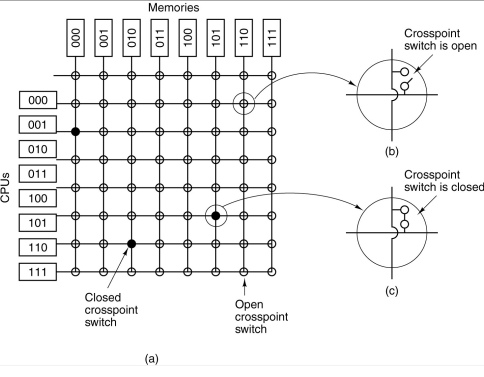
\includegraphics[scale=0.7]{04-ArchitettureParallele/crossbar.png}
    \caption{Nell’esempio, tre switch sono chiusi, e connettono le coppie CPU-
memoria (001-000), (101-101) e (110-010).}
\end{figure}

\dfn{UMA a Crossbar Switch}{
  È possibile configurare gli switch  in modo che ciascuna CPU possa connettersi a ciascun banco di memoria. Il numero di switch necessari per realizzare questo schema però
cresce quadraticamente col numero di CPU (memorie) coinvolte:
n CPU e $4n$ memorie richiedono $n^2$ switch. La cosa è accettabile per sistemi di media grandezza (vari sistemi
multiprocessore della Sun usano questo schema), ma certamente
non è usabile in un sistema con 256 CPU (sarebbero
necessari $256^2$ switch).
}

\nt{Quando il numero di CPU è alto, si può usare un sistema
basato su switch bidirezionali con due ingressi e due uscite: in
questi switch ciascun ingresso può essere rediretto su
ciascuna uscita.}

\begin{figure}[h]
    \centering
    \begin{minipage}{0.45\textwidth}
        \centering
        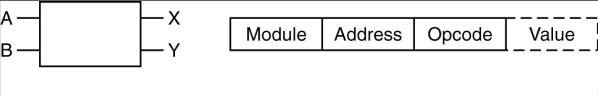
\includegraphics[scale=0.5]{04-ArchitettureParallele/bi.png}
        \caption{Sistema di switch bidirezionali.}
    \end{minipage}
    \hfill
    \begin{minipage}{0.45\textwidth}
        \centering
        
\includegraphics[scale=0.25]{04-ArchitettureParallele/bi2.png}
        \caption{Switch bi-???}
    \end{minipage}
\end{figure}

\paragraph{Nei sistemi UMA che usano switch bidirezionali i messaggi
scambiati tra CPU e memoria sono fatti di quattro parti:}

\begin{itemize}
  \item \fancyglitter{Module}: quale memoria usare, quale CPU richiede il dato. 
  \item \fancyglitter{Address}: specifica un indirizzo all'interno del modulo di memoria. 
  \item \fancyglitter{Opcode}: l'operazione da eseguire. 
  \item \fancyglitter{Value} (opzionale): il valore da scrivere nel caso di write.
\end{itemize}

\nt{Lo switch può essere programmato in modo da analizzare il
Module e determinare su quale output instradare il messaggio.}

\begin{figure}[h]
    \centering
    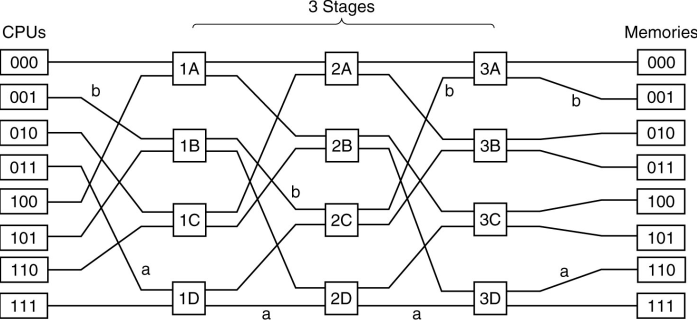
\includegraphics[scale=0.5]{04-ArchitettureParallele/Omega.png}
    \caption{Gli switch 2 x 2 possono essere usati in molti modi per costruire reti
a commutazione a più stadi. Un semplice esempio è il modello di
rete omega.}
\end{figure}

\begin{itemize}
  \item Nell’esempio, 8 CPU sono connesse a 8 memorie, usando in tutto
12 switch in tre stadi. In generale, $n$ CPU e $n$ memorie richiedono
$log_2n$ stadi, con $\frac{n}{2}$ switch per stadio, per un totale di $(\frac{n}{2})log_2n$
switch: molto meglio che nel caso dei crossbar switch ($n^2$). 
\item La CPU 011
vuole leggere un dato nel modulo di RAM 110. La CPU invia una
READ allo switch 1D con Module = 110 -- 011. 
\item Lo switch preleva il bit più significativo (quello più a sinistra) e lo
usa per l’instradamento: 0 instrada la richiesta sull’output superiore,
1 instrada la richiesta sull’output inferiore. 
\item Lo switch 2D si comporta allo stesso modo: analizza il secondo bit
più significativo (quello centrale) e instrada la richiesta verso 3D. 
\item Infine, il bit meno significativo viene usato per l’ultimo
instradamento, verso il modulo 110 (percorso a nella figura). 
\item A questo punto, il dato letto deve essere reinstradato alla CPU 011:
viene usato il suo “indirizzo”, leggendo però i bit da destra verso
sinistra. 
\item Allo stesso tempo, la CPU 001 vuole eseguire una WRITE nel
modulo 001. Avviene un processo simile a quello visto (percorso b
nella figura). Siccome i percorsi a e b non usano gli stessi switch, le
due richieste possono procedere in parallelo. 
\end{itemize}

\nt{Al contrario di quello che accade con le reti che usano crossbar
  switch, le reti omega sono \fancyglitter{reti bloccanti}: non tutte le sequenze di
richieste possono essere servite contemporaneamente.}

\subsection{NUMA}

I sistemi UMA a bus singolo sono limitati dal numero di processori,
e per connettere più processori è necessario dell’hardware
comunque costoso. Allo stato attuale, non è conveniente costruire
sistemi UMA con più di qualche centinaio di processori. Per costruire sistemi più grandi è necessario accettare un
compromesso: che non tutti i moduli di memoria abbiano
lo stesso tempo di accesso rispetto a ciascuna CPU.

\dfn{NUMA}{ 
Non Uniform Memory Access (NUMA) è un tipo di architettura in cui la memoria fisica è distribuita tra le varie CPU e quindi i tempi di accesso ai dati variano a seconda che siano nella RAM locale o in una remota.
}

\nt{Questi sistemi vengono anche chiamati DSM (Distribuited Shared-Memory).}

\begin{figure}[h]
    \centering
    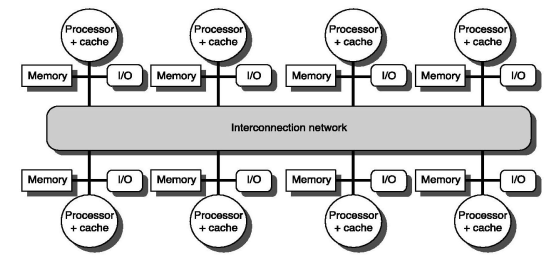
\includegraphics[scale=0.6]{04-ArchitettureParallele/NUMA.png}
    \caption{Schema NUMA.}
\end{figure}

\clm{}{}{
  \begin{itemize}
    \item Come per i UMA, nei sistemi NUMA tutte le CPU vedono lo stesso
spazio di indirizzamento ma, ogni processore è dotato di una sua
propria memoria locale, vista anche da tutti gli altri processori. 
\item Al contrario dei sistemi UMA quindi, nei sistemi NUMA l’accesso
ai moduli di memoria locale è più veloce dell’accesso ai moduli di
memoria remoti. 
\item Come conseguenza, i programmi scritti per sistemi UMA possono
comunque girare senza dover apportare alcun cambiamento su
macchine NUMA, possibilmente con prestazioni diverse a causa dei
diversi tempi di accesso ai vari moduli remoti di RAM.
\item Poiché le macchine NUMA hanno uno spazio di indirizzamento
logico unico visto da tutte le CPU, mentre la memoria fisica è in
realtà suddivisa tra i vari processori, emerge il concetto di memoria
locale e remota.   
\end{itemize}
}

\paragraph{Esistono due tipi di sistemi NUMA:}

\begin{itemize}
  \item \fancyglitter{Non-Caching NUMA (NC-NUMA)}. 
  \item \fancyglitter{Cache-Coherent NUMA (CC-NUMA)}.
\end{itemize}

\dfn{NC-NUMA}{
  In un sistema NC-NUMA i processori non hanno cache locale. Ogni accesso alla memoria è gestito da una MMU modificata, che
controlla se la richiesta è diretta alla memoria locale o a un modulo
remoto, nel qual caso la richiesta viene instradata al nodo che
contiene il dato richiesto. 
}

\nt{I programmi che usano dati remoti risulteranno più lenti che se i dati fossero memorizzati nella memoria locale.}

\clm{}{}{
  \begin{itemize}
    \item Nei sistemi NC-NUMA il problema della coerenza
della cache è automaticamente risolto perché non c’è nessuna forma
di caching: ogni dato della memoria è presente esattamente in una
locazione ben precisa.
\item Rimane il problema dell’inefficienza dell’accesso alla memoria
remota. Per questo, le macchine NC-NUMA possono usare software
elaborato per spostare le pagine di memoria da un modulo all’altro
in modo da minimizzare gli accessi remoti e massimizzare le
prestazioni. 
\item Un page scanner può attivarsi ogni pochi secondi, esaminare le
statistiche sull’indirizzamento della memoria, e spostare le pagine
da un modulo all’altro per cercare di migliorare le prestazioni.
\item Nei sistemi NC-NUMA, ogni processore può avere anche
una memoria locale privata e una cache, e solo i dati privati del
processore (ossia quelli nella memoria locale privata) possono
risiedere nella cache. Questa soluzione aumenta ovviamente le prestazioni di ciascun
processore.
  \end{itemize}
}

\dfn{CC-NUMA}{
  Aggiungere il caching diminuisce ovviamente i tempi di accesso
ai dati remoti, ma introduce il problema della coerenza della cache.
Un modo di garantire la coerenza sarebbe ovviamente lo snooping
sul bus di sistema, ma questa tecnica diventa troppo inefficiente
oltre un certo numero di CPU, ed è comunque troppo difficile da
implementare nei sistemi che non usano un bus comune di
interconnessione. 

L’approccio più usato per costruire sistemi CC-NUMA con molte
CPU assicurando la coerenza della cache è noto come schema o
protocollo \newfancyglitter{directory-based} (multiprocessor).
L’idea di base è di associare ad ogni nodo del sistema una directory
per le linee della sua RAM: un database che registra in quale cache
di quale nodo si trova ogni linea, e qual è il suo stato.
}

\clm{}{}{
  \begin{itemize}
    \item Quando viene indirizzata una linea di RAM, la directory del nodo a
cui quella linea appartiene viene interrogata per sapere se la linea si
trova in qualche cache e se questa sia stata modificata rispetto alla
copia in RAM. 
\item Poiché una directory viene interrogata ogni volta che una istruzione
accede la corrispondente memoria, deve essere implementata con un
hardware molto veloce, per esempio una memoria associativa.
\item Come esempio di protocollo directory based, consideriamo un
sistema con 256 nodi, ognuno formato da una CPU e una RAM
locale da 16 MB. Ci sono in tutto 232 = 4 GB di RAM, e ogni nodo contiene 218 linee
da 64 byte ciascuna (218 x 26 = 224 = 16 MB). Lo spazio di indirizzamento è unico, col nodo zero che contiene la
memoria con indirizzi da 0 a 16 MB, il nodo 1 la memoria con
indirizzi da 16 a 32 MB, e così via. Un indirizzo fisico è quindi scritto su 32 bit (gli 8 bit più significativi indirizzano di fatto il numero del nodo a
cui appartiene il banco di RAM che contiene il dato indirizzato, i successivi 18 bit indicano la linea indirizzata all’interno del banco
da 16 MB e i restanti 6 bit meno significativi indirizzano il byte all’interno della
linea).
  \end{itemize}
}

\begin{figure}[h]
    \centering
    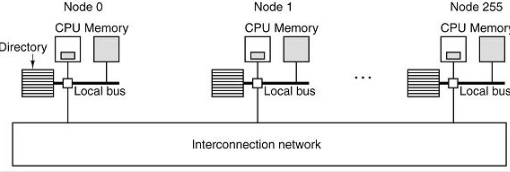
\includegraphics[scale=0.7]{04-ArchitettureParallele/CC_NUMA.png}
    \caption{Esempio di CC-NUMA.}
\end{figure}

\paragraph{In un sistema reale, l'architetturà directory-based:}

\begin{itemize}
  \item Le linee di RAM possono essere contemporaneamente nella cache di più nodi. 
  \item Si tiene traccia del fatto che una cache line sia stata modificata o meno e si possono limitare le comunicazioni tra CPU e memorie. 
  \item Se una cache line non è stata modificata la linea originale in RAM è ancora valida e una read da una CPU remota per quellls line può essere soddisfatta dalla RAM stessa, senza dover andare a recuperare la linea della cache che ne contiene una copia.
\end{itemize}

\subsection{Sincronizzazione tra Processi}

In un sistema monoprocessore, i vari processi si sincronizzano fra
loro usando opportune system call o costrutti del linguaggio in uso:
semafori, regioni critiche condizionali, monitors. Questi meccanismi di sincronizzazione sono costruiti a partire da
opportune primitive di sincronizzazione hardware: spesso una
istruzione macchina non interrompibile in grado di prelevare e
modificare un valore, o di scambiare il contenuto di un registro e
una cella di memoria. In un sistema multiprocessore abbiamo bisogno di primitive di
sincronizzazione simili: i processi vedono un unico spazio di
indirizzamento e la sincronizzazione deve avvenire sfruttando
questo spazio comune, e non meccanismi a scambio di messaggi.

\begin{figure}[h]
    \centering
    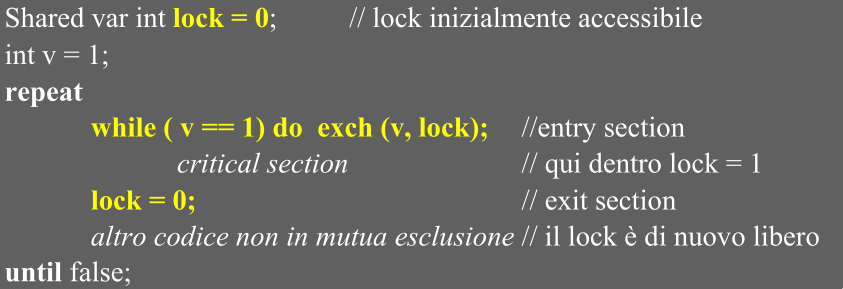
\includegraphics[scale=0.4]{04-ArchitettureParallele/Lock.png}
    \caption{Spin lock, il processo cicla sulla variabile di lock fino a quando non la trova libera.}
\end{figure}

\nt{In questo caso è presente un problema di \fancyglitter{attesa attiva} per cui i test della variabile sprecano il quanto di tempo dei processi.}

\subsubsection{}

Tuttavia, in un ambiente in cui i processi che usano una variabile
condivisa per sincronizzarsi possono girare su CPU diverse,
l’atomicità delle istruzioni di sincronizzazione non è sufficente. 

\qs{}{
  Su un processore, l’istruzione atomica sarà eseguita senza
interruzioni, ma che succede sugli altri processori? Avrebbe senso disabilitare tutte le operazioni sulla memoria dal
momento in cui una primitiva di sincronizzazione viene avviata a
quando ha finito di modificare la variabile di sincronizzazione?
}

\paragraph{Risposta:} Funzionerebbe, ma questo danneggerebbe le operazioni delle CPU
non coinvolte nella sincronizzazione. La soluzione adottata in molti processori usa una coppia di
istruzioni macchina eseguite una dopo l’altra. La prima istruzione cerca di scrivere in uno dei registri della CPU
il valore della variabile condivisa. La seconda istruzione cerca di modificare la variabile condivisa, e
restituisce un valore da cui si può capire
se la coppia di istruzioni è stata eseguita in modo atomico,
il che in un sistema multiprocessore, significa: 


\begin{itemize}
  \item Nessun altro processo attivo su qualsiasi processore ha modificato
il valore della variabile usata per la sincronizzazione prima della
terminazione della seconda istruzione della coppia.
\item Durante l’esecuzione delle due istruzioni non si è verificato alcun
context switch nel processore che le ha eseguite.
\end{itemize}

\ex{Sincronizzazione}{
  Sia $[0(R1)]$ il valore della cella di memoria di indirizzo $0(R1)$,
usata come variabile condivisa di sincronizzazione.
\begin{center}
  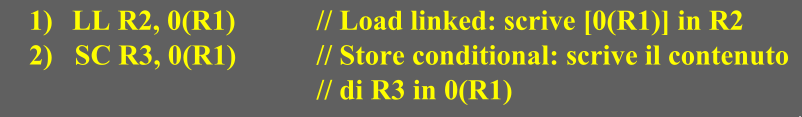
\includegraphics[scale =0.55]{04-ArchitettureParallele/ex1.png}
\end{center}
L’esecuzione delle due istruzioni rispetto a 0(R1) è vincolata a ciò
che accade tra l’esecuzione delle due istruzioni:

\begin{itemize}
  \item Se $0(R1)$ viene modificata da un altro processo prima della
terminazione della SC, la SC fallisce, ossia:
$0(R1)$ non viene modificata dalla SC e viene scritto 0 in R3.
Se invece la SC non fallisce, allora:
$R3$ viene copiato in $0(R1)$ e in $R3$ viene scritto 1.
  \item Analogamente, se la CPU su cui la coppia di istruzioni viene
eseguita esegue un context switch tra le due istruzioni, la SC
fallisce, con gli stessi effetti del punto 1.
\end{itemize}
Una exchange “atomica” tra R4 e
0( R1) in un sistema multiprocessore (simile ad uno spin lock):
\begin{center}
  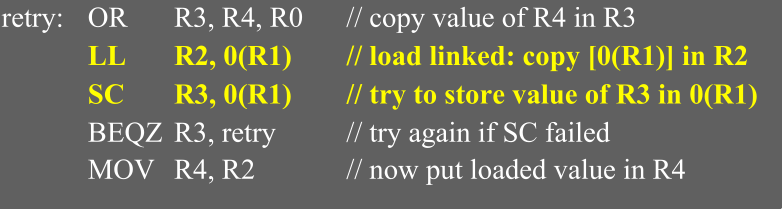
\includegraphics[scale =0.55]{04-ArchitettureParallele/ex2.png}
\end{center}
Quando la MOV viene eseguita, $R4$ e $0(R1)$ sono stati scambiati in
modo “atomico”, e si è certi che il contenuto di $0(R1)$ non è stato
modificato da altri processi prima del completamento della
exchange. Chiamiamo EXCH l’operazione eseguita da questo
codice.

Una volta in possesso di un’operazione atomica EXCH, la si può
usare per implementare spin locks: accessi ad una sezione critica
che ogni processore cerca di acquisire ciclando sulla variabile di
lock, che controlla appunto l’accesso mutuamente esclusivo. 
}
\subsubsection{}
Se le CPU non sono dotate di cache, la variabile di lock viene
ovviamente tenuta in memoria: un processore cerca di acquisire il
lock con una exchange atomica, e verifica se il lock è libero. 
Se le CPU sono dotate di cache allora è presente un meccanismo per
mantenere la coerenza della cache, e ogni processore coinvolto nella
sincronizzazione userà la copia della variabile di lock che ha portato
nella propria cache.
Questo rende il meccanismo dello spin lock più efficiente, perché
tutte le operazioni dei vari processori che cercano di acquisire il
lock operano sulle rispettive cache, in modo più efficiente. Il codice dello spin lock va però modificato: ogni processore esegue
una read sulla copia in cache del lock, fino a quando non vede che il
lock è libero. A questo punto tenta di acquisire il lock con la exchange atomica.

\ex{Sincronizzazione con Cache}{
\begin{center}
  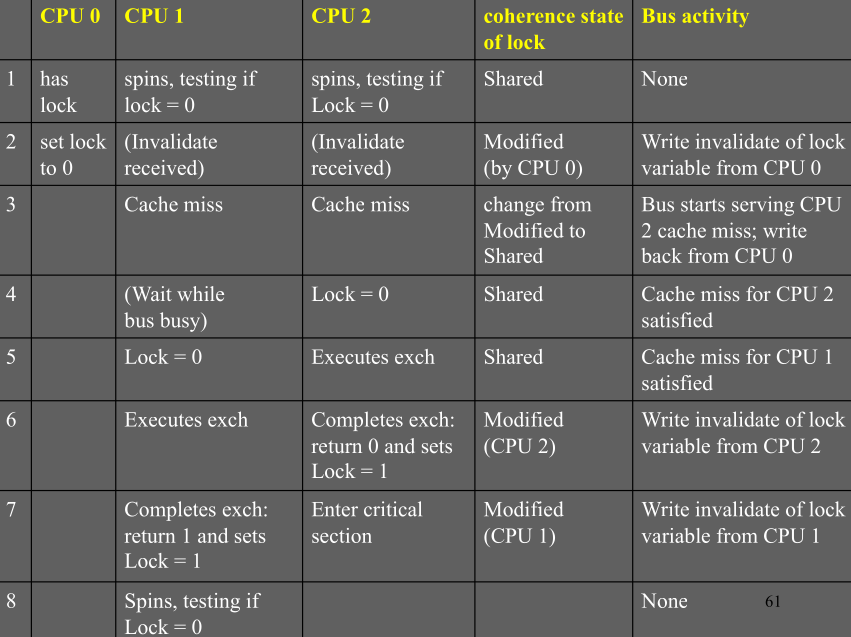
\includegraphics[scale =0.45]{04-ArchitettureParallele/SinCache.png}
\end{center}
\begin{enumerate}
  \item CPU 0 ha il lock, CPU 1 e CPU 2 testano ripetutamente la copia della variabile di
lock nelle rispettive cache. 
\item CPU 0 rilascia il lock, e il MESI genera un segnale di invalidazione della copia
della variabile di lock nelle cache di CPU 1 e CPU 2. 
\item Le LOAD eseguite da CPU 1 e CPU 2 generano un cache miss, e il MESI
interviene per recuperare il valore aggiornato della variabile di lock che si
trova nella cache di CPU 0 e aggiornare la RAM. 
\item Il MESI serve il cache miss di CPU 2, CPU 1 deve aspettare (l’ordine con cui
vengono servite le richieste segue l’ordine con cui sono state ricevute). 
\item CPU 2 inizia ad eseguire la EXCH, mentre viene servito il cache miss di CPU 1. 
\item Anche CPU 1 inizia ad eseguire la EXCH, ma nel frattempo CPU 2 completa
la sua EXCH modificando il valore del lock nella sua cache. Il MESI deve
intervenire per invalidare la copia del lock nella cache di CPU 1. 
\item CPU 1 completa la sua EXCH ma trova lock = 1 (settato da CPU 2) dunque il
MESI interviene di nuovo per invalidare le copie del lock nelle varie cache
(questo “invalidate” è inutile se non ci sono altre CPU con il lock in cache). 
\item CPU 1 torna a testare il valore del lock in attesa che venga modificato da CPU 2.
\end{enumerate}
}

\nt{La tecnica vista funziona senza troppo overhead (ossia, l’attesa
attiva non spreca troppi cicli di clock) solo per sistemi con poche
CPU, o perlomeno con poche CPU coinvolte nel tentativo di
acquisire il lock. Quando il numero di CPU coinvolte nel tentativo di acquisire il lock
può essere “alto” (diciamo, da 10 CPU in su), vengono usati
meccanismi un pò più sofisticati, ma sempre basati sulle primitive
di sincronizzazione LL e SC già viste.}

\subsection{Modelli di Consistenza della Memoria}

In un sistema multiprocessore tutte le CPU hanno accesso a uno
spazio di memoria primaria condiviso, e quando una CPU modifica
una cella di memoria, un’altra CPU vedrà prima o poi quella
modifica.

\qs{}{In che ordine una CPU deve vedere le modifiche effettuate sulle
celle di RAM effettuate dalle altre CPU?}

\paragraph{Risposta:} La questione non è banale, dato che il sistema può essere costituito
da centinaia di CPU e centinaia o migliaia di banchi di memoria, il
tutto messo in comunicazione da reti a tipologia diversa, con
conseguenti tempi variabili di completamento delle scritture/letture
in RAM. Persino in un semplice sistema UMA con poche CPU che si
affacciano su un unico bus di comunicazione, il problema esiste.

\dfn{Consistenza stretta}{
  La forma più ovvia (ma non implementabile) di consistenza è che qualsiasi lettura a una
cella X restituisce sempre il valore dovuto alla scrittura più recente
effettuata nella stessa cella.
}

\clm{}{}{
  \begin{itemize}
    \item Sfortunatamente, è anche la forma di consistenza più difficile e
inefficiente da garantire: è necessaria un’interfaccia tra le varie
CPU e la memoria che gestisca tutte le richieste di accesso alla
memoria stessa in modalità first come first served. 
\item La memoria diviene così un collo di bottiglia che rallenta in modo
inaccettabile un sistema costruito per lavorare il più possibile in
parallelo.
  \end{itemize}
}

\dfn{Consistenza del Processore}{
  \begin{itemize}
    \item \newfancyglitter{Le scritture da parte di una qualsiasi CPU sono viste dalle altre
CPU nell’ordine in cui sono state avviate}: se CPU 1 scrive A, B e
C in una locazione var, una CPU 2 che legga var in sequenza più
volte leggerà prima A, poi B e poi C.
\item \newfancyglitter{Per ogni locazione di memoria, qualsiasi CPU vede tutte le
scritture effettuate da ogni singola CPU in quella locazione
nello stesso ordine}.
  \end{itemize}
}

\nt{Diverse CPU che leggano più volte var potranno leggere sequenze
diverse. Ciò che viene garantito è che nessuna CPU vedrà una
sequenza in cui, per esempio, B viene prima di A o Z viene prima di
Y: l’ordine in cui ciascuna CPU esegue le sue scritture, viene
visto allo stesso modo da tutte le altre.}

\section{Multicomputer a scambio di
messaggi (e miscellanea)}

\subsection{Introduzione}

Il limite alla scalabilità dei sistemi multiprocessore è dovuto alla
difficoltà di connettere fra loro molti nodi (single o multi-core)
fornendo a ciascuno la visibilità dell’intero spazio di memoria. Anche risolvendo il problema della rete di connessione, l’uso di una
memoria condivisa in cui centinaia di CPU stanno cercando di
accedere alle stesse variabili crea un collo di bottiglia che limita
fortemente la scalabilità di questo tipo di architetture. 
Nei sistemi multicomputer i programmi che girano su ciascun nodo
interagiscono scambiandosi informazioni attraverso primitive come
SEND e RECEIVE anziché con istruzioni come LOAD e STORE. Ogni nodo del sistema è composto di una o pochi processori, ormai
sempre multi-core, della RAM condivisa solo dai core locali,
eventualmente un disco (e/o altri dispositivi di I/O), e un processore
per la comunicazione attraverso una rete di interconnessione.

\dfn{NORMA}{
  Quando c’è bisogno di una potenza computazionale maggiore di
quella che possono fornire i sistemi a memoria condivisa, è
necessario ricorrere ad architetture in cui i vari nodi comunicano
solo attraverso lo scambio di messaggi, e non esiste uno spazio di
indirizzamento comune. A causa di questa caratteristica, queste
architetture sono a volte chiamate \newfancyglitter{NO Remote Memory Access}
(NORMA).
}

\subsection{Massively Parallel Processor (MPP)}

Le architetture MPP sono sistemi con un costo dell’ordine dei
milioni o decine di milioni di dollari, usati per applicazioni
scientifiche, finanziarie e militari. Gli MPP sono tipicamente costituiti da centinaia di migliaia o
milioni di nodi formati da processori standard o prodotti
appositamente, connessi da una rete privata ad alte prestazioni. Gli MPP hanno di solito anche una alta capacità di I/O, dovuta al
tipo di problemi trattati che richiedono la capacità di processare
grosse quantità di dati (dell’ordine dei terabytes) e di spostarli
velocemente da una macchina all’altra. Spesso usano software di gestione del sistema appositamente
sviluppato per la sincronizzazione e la comunicazione fra i processi:
librerie dedicate e/o sistema operativo. Infine, gli MPP devono avere una alta tolleranza ai guasti, che non
possono che essere frequenti, dato l’elevatissimo numero di
processori, banchi di memoria, e dischi coinvolti.

\nt{Devono così essere previsti specifici meccanismi hardware e
software per monitorare il sistema, gestire i guasti, ed evitare che il
lavoro fatto fino a quel punto vada perso. Questi sistemi sono prodotti in quantità ovviamente limitate, così
che non esistono dei principi generali di progettazione: ogni sistema
ha le sue proprie peculiarità.}

\dfn{BlueGene}{
  Il progetto BlueGene dell’IBM nasce nel 1999 con l’obiettivo di
produrre un supercomputer adatto a risolvere problemi che
richiedono un elevato sforzo computazionale: nell’analisi della
struttura delle proteine umane, nei modelli climatici, in campo
astronomico, finanziario e militare. L’idea era quella di costruire non solo il sistema più veloce in
termini di potenza di calcolo (teraflops), ma anche il più efficiente
in termini di teraflops/\$, teraflops/watt, teraflops/$m^3$.
}

\begin{figure}[h]
    \centering
    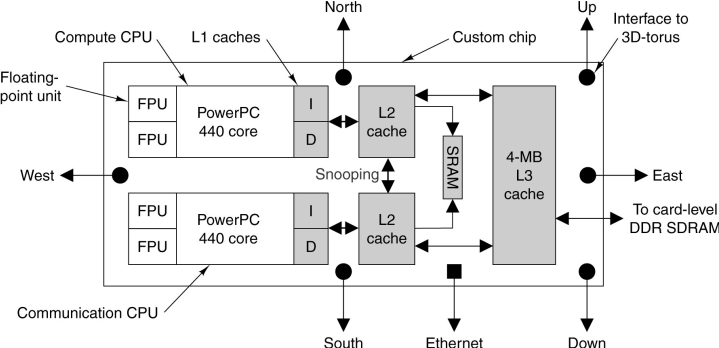
\includegraphics[scale=0.4]{04-ArchitettureParallele/BlueGene.png}
    \caption{Nel progetto iniziale, il cuore di BlueGene era un chip (prodotto a
partire dalla metà del 2003) formato da due PowerPC 440 con un
clock a “soli” 700 MHz.}
\end{figure}

\clm{}{}{
  \begin{itemize}
    \item Il PowerPC 440 è un processore superscalare, usato principalmente
in sistemi embedded, in grado di avviare fino a 4 istruzioni anche
floating point) per ciclo di clock. La versione usata in BlueGene è
stata arricchita con istruzioni FP di tipo vettoriale. 
\item I due core su ogni chip sono identici, ma uno è usato per le
computazioni vere e proprie, e l’altro per le comunicazioni tra i vari
nodi del sistema. 
\item Ogni coppia di core ha a disposizione 512MB di RAM privata
(condivisa dai due core), estendibili fino a 2 GB. Per la coerenza
delle cache tra i due core viene usata una logica di snooping.
  \end{itemize}
}

\paragraph{Progettazione del BlueGene:}

\begin{itemize}
  \item Una scheda custom ospita due chip e la RAM per ciascun chip. 
  \item 16 schede custom sono montate su una motherboard, per un totale
di 32 chip (ossia 32 core per la computazione) e almeno 16GB. 
\item 32 motherboard sono ospitate in un cabinet, per un totale di 1024
core per la computazione. 
\item Infine, un sistema
completo è formato da
64 cabinet, per un totale
di 65,536 core per la
computazione e almeno
32TB di RAM.
\end{itemize}

\begin{figure}[h]
    \centering
    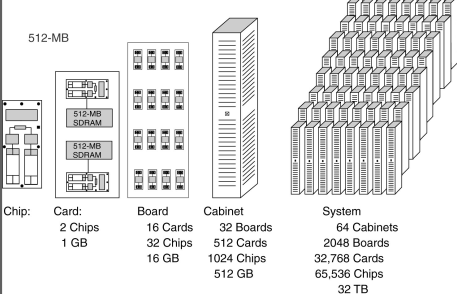
\includegraphics[scale=0.4]{04-ArchitettureParallele/BG.png}
    \caption{Il sistema BlueGene.}
\end{figure}
\subsubsection{}

Ogni core ha accesso diretto solo alla propria RAM, e
che non esistono dischi “locali”: Il sistema ha invece 1024 nodi di
I/O, connessi ai dischi e ad altre periferiche. La rete di interconnessione tra i nodi
è un toroide a tre dimensioni:
Un toroide a due dimensioni è una griglia
con i nodi ai lati connessi fra loro. In un toroide 3D, ogni nodo è all’intersezione
di 3 assi anziché 2, e ha due vicini ai due lati di ogni asse. Ogni chip comunica quindi con sei vicini, con una connessione
punto a punto ad una velocità di 1,4 Gbit/sec, con una ampiezza di
banda totale (la quantità di informazione che può essere spostata
nell’intero sistema nell’unità di tempo) di 275 terabit/sec. 

La comunicazione tra i nodi è sostanzialmente a commutazione di
pacchetto, ma il sistema è connesso anche attraverso altre reti (tra
cui una Gigabit Ethernet), per gestire la manutenzione e la
comunicazione con i dispositivi di memorizzazione di massa
(dischi e sistemi a nastro magnetico). Su ogni chip gira un SO molto semplice, appositamente
sviluppato, che supporta un solo utente ed un solo processo
suddiviso in due thread: uno per ciascun core del chip. Questa
soluzione garantisce alte prestazioni e bassi errori software.
Attraverso software opportuno, il sistema è in grado di eseguire dei
checkpoint, ai quali l’intero stato della computazione viene salvato
su disco. In caso di crash del sistema, la computazione può
riprendere dall’ultimo check point.

\nt{Oggigiorno i successori dei BlueGene raggiungono ormai le
centinaia di PetaFLOPS e combinano processori custom e GPU (se ne parlerà nel sesto capitolo)
per massimizzare la potenza di calcolo.}

\subsection{Cluster Of Workstation (COW)}

Un cluster è tipicamente formato da un insieme di macchine
connesse in rete. In genere, le unità
computazionali di un MPP sono tutte uguali, e sono
“impacchettate” in modo molto “denso” in una struttura
progettata appositamente. I processori comunicano fra loro mediante una rete ad alte
prestazioni, spesso progettata specificamente per quella architettura. La singola unità computazionale non potrebbe “funzionare dasola”. Al contrario, un cluster è innanzi tutto costituito da macchine che
possono essere anche molto diverse fra loro: PC e workstations con
processori diversi. In alcuni casi, ciascuna unità computazionale costituisce un sistema
che potrebbe anche funzionare da solo (al massimo mancano il
video e la tastiera/mouse). I vari nodi sono connessi da una rete non progettata esplicitamente
per quell’applicazione: una rete Ethernet o anche Internet. Ancor meno che con i MPP, non esiste un criterio di progettazione
specifico per i cluster, e il numero di nodi connessi è estremamente
variabile: si va da qualche PC ai milioni di core di un sistema
distribuito geograficamente come Google. 

\subsection{Processori Vettoriali}

La quantità di hardware necessaria per eseguire in parallelo più
istruzioni cresce più che linearmente (più o meno quadraticamente)
con il numero di istruzioni eseguite in parallelo. Questo limita praticamente il numero di istruzioni avviabili per
ciclo di clock e il numero di stadi di una pipeline. 

\dfn{Processori Vettoriali}{
I \newfancyglitter{processori vettoriali}, commercializzati a partire da metà anni 70
(i più famosi sono certamente i vari modelli prodotti dalla Cray),
rappresentano una alternativa allo sfruttamento dell’ILP tipico dei
classici processori superscalari – multiple issue moderni. Queste architetture mettono a disposizione istruzioni che lavorano
su vettori di dati, ossia, in sostanza, su array di numeri.
L’istruzione vettoriale è quindi equivalente a un intero loop in cui
ad ogni iterazione verrebbe calcolato uno dei 64 elementi di output,
verrebbero aggiornati gli indici e si salterebbe indietro all’inizio del
ciclo per operare sull’elemento successivo.
}

\clm{}{}{
  Le istruzioni vettoriali hanno quindi delle importanti caratteristiche: 
  \begin{itemize}
    \item \fancyglitter{Una singola istruzione vettoriale specifica molto lavoro,
      equivalente a eseguire un intero loop}: In particolare, una istruzione può rappresentare decine di operazioni
più semplici, e intere unità funzionali posso essere tenute
completamente occupate prelevando ed eseguendo una sola di tali
istruzioni (invece che preoccuparsi di prelevare e lanciare molte
istruzioni potenzialmente dipendenti tra loro ad ogni ciclo di clock). 
\item \fancyglitter{L’uso di una istruzione vettoriale indica che la computazione
di ogni elemento del vettore risultato è indipendente dalla
computazione di altri risultati nel vettore}: Come conseguenza, l’hardware della CPU non deve controllare
nessun data hazard all’interno di una istruzione vettoriale, e gli
elementi del vettore possono essere elaborati usando un array di
unità funzionali in parallelo. 
\item \fancyglitter{È necessario controllare le alee tra due istruzioni vettoriali solo
una volta per ogni vettore operando, e non per ogni elemento
dei due vettori}: La logica di controllo è quindi molto più semplice, a parità di potere
espressivo delle istruzioni.
\item \fancyglitter{Le istruzioni vettoriali accedono di solito a locazioni adiacenti di
memoria, quelle che ospitano i vari elementi del vettore}: Gli accessi alla memoria (sia questa la RAM o la cache) sono in
generale più efficienti, perché è più probabile che valga il principio
di località.
\item \fancyglitter{Un intero loop viene sostituito da un’unica istruzione vettoriale}: Come conseguenza, scompaiono tutti gli hazard sul controllo, e la
necessità di gestire il branch prediction. 
  \end{itemize}
}

\nt{I processori vettoriali trovano un naturale impiego in vari campi
scientifici e industriali in cui sia necessario manipolare grandi
quantità di dati che hanno una naturale “forma” vettoriale: ad
esempio, le previsioni metereologiche, simulazioni di crash test,
applicazioni multimediali.}


\begin{figure}[h]
    \centering
    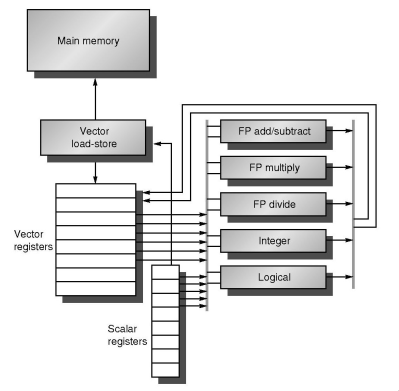
\includegraphics[scale=0.4]{04-ArchitettureParallele/Vet.png}
    \caption{Architettura di base di un processore vettoriale.}
\end{figure}

\paragraph{Un processore vettoriale è composto da:}

\begin{itemize}
  \item Registri vettoriali: 8 registri vettoriali, ciascuno dei quali contiene 64 elementi da 32 o 64 bit ciascuno. 
  \item Unità funzionali vettoriali: Ogni unità è pipelined, è può far
partire una nuova operazione ad ogni ciclo di clock. Una unità di
controllo verifica gli eventuali conflitti nell’uso delle unità
funzionali (hazard strutturali) e nell’accesso ai registri (Hazard sui
dati). 
\item Unità vettoriali load-store: Possono operare in modo tale da
spostare l’intero contenuto di più celle adiacenti di RAM nei
registri vettoriali, e viceversa.
\item Registri scalari. Che possono essere usati per calcolare indirizzi di
RAM o per eseguire operazioni tra vettori e scalari.
\end{itemize}

\qs{}{Perché i processori vettoriali non hanno preso il sopravvento sulle
classiche architetture superscalari?}

\paragraph{Risposta:} Innanzi tutto, i processori vettoriali hanno una architettura
inerentemente più complessa, che limita verso l’alto la velocità del
clock: nel 2001 la più veloce architettura vettoriale aveva un clock
di 500 MHz. La complessità dell’architettura è dovuta proprio al modo in cui
operano i processori vettoriali. Come conseguenza, la domanda del mercato è sempre rimasta
limitata e non sono state possibili produzioni su larga scala che
ne avrebbero abbattuto i prezzi. Per contro, l’aumento delle prestazioni delle classiche CPU
superscalari degli anni 80 e 90 ha permesso ai processori
tradizionali di diminuire le differenze rispetto alle prestazioni dei
processori vettoriali anche su problemi tipicamente “vettoriali”. Per tutte queste ragioni, i processori vettoriali sono ormai diventati
prodotti di nicchia. Tuttavia l’esperienza progettuale dei processori
vettoriali è stata almeno parzialmente trasferita nei processori
superscalari moderni. Infatti, molte applicazioni multimediali contengono codice che può
essere naturalmente vettorizzato, e molti processori moderni hanno
arricchito il loro set di istruzioni macchina con estensioni
multimediali che ricalcano lo stile delle istruzioni vettoriali.

